%%%%%%%%%%%%%%%%%%%%%%%%%%%%%%%%%%%%%%%%%
% Short Sectioned Assignment
% LaTeX Template
% Version 1.0 (5/5/12)
%
% This template has been downloaded from:
% http://www.LaTeXTemplates.com
%
% Original author:
% Frits Wenneker (http://www.howtotex.com)
%
% License:
% CC BY-NC-SA 3.0 (http://creativecommons.org/licenses/by-nc-sa/3.0/)
%
%%%%%%%%%%%%%%%%%%%%%%%%%%%%%%%%%%%%%%%%%

%----------------------------------------------------------------------------------------
%	PACKAGES AND OTHER DOCUMENT CONFIGURATIONS
%----------------------------------------------------------------------------------------

\documentclass[paper=a4, fontsize=11pt]{scrartcl} % A4 paper and 11pt font size
\usepackage[shortlabels]{enumitem}
\usepackage{float}
\usepackage{ctex}
\usepackage{amssymb}
\usepackage{hyperref}
\usepackage{listings}
\usepackage[T1]{fontenc} % Use 8-bit encoding that has 256 glyphs
\usepackage{fourier} % Use the Adobe Utopia font for the document - comment this line to return to the LaTeX default
\usepackage[english]{babel} % English language/hyphenation
\usepackage{amsmath,amsfonts,amsthm} % Math packages

\usepackage{lipsum} % Used for inserting dummy 'Lorem ipsum' text into the template

\usepackage{sectsty} % Allows customizing section commands
%\allsectionsfont{\centering \normalfont\scshape} % Make all sections centered, the default font and small caps
\usepackage{mathrsfs}
\usepackage{fancyhdr} % Custom headers and footers
\usepackage{algorithm}
\usepackage[noend]{algpseudocode}
\algnewcommand\Break{\textbf{break}}

\usepackage{scrextend} % for addmargin
\usepackage{subcaption}
\graphicspath{{p3/}}
%\usepackage{algorithmic}
\usepackage[noend]{algpseudocode}
\usepackage{listings}
\pagestyle{fancyplain} % Makes all pages in the document conform to the custom headers and footers
\fancyhead{} % No page header - if you want one, create it in the same way as the footers below
\fancyfoot[L]{} % Empty left footer
\fancyfoot[C]{} % Empty center footer
\fancyfoot[R]{\thepage} % Page numbering for right footer
\renewcommand{\headrulewidth}{0pt} % Remove header underlines
\renewcommand{\footrulewidth}{0pt} % Remove footer underlines
\setlength{\headheight}{13.6pt} % Customize the height of the header

\numberwithin{equation}{section} % Number equations within sections (i.e. 1.1, 1.2, 2.1, 2.2 instead of 1, 2, 3, 4)
\numberwithin{figure}{section} % Number figures within sections (i.e. 1.1, 1.2, 2.1, 2.2 instead of 1, 2, 3, 4)
\numberwithin{table}{section} % Number tables within sections (i.e. 1.1, 1.2, 2.1, 2.2 instead of 1, 2, 3, 4)

\setlength\parindent{0pt} % Removes all indentation from paragraphs - comment this line for an assignment with lots of text

\newtheorem{theorem}{Theorem}[section]
\newtheorem{corollary}{Corollary}[theorem]
\newtheorem{lemma}[theorem]{Lemma}

%----------------------------------------------------------------------------------------
%	TITLE SECTION
%----------------------------------------------------------------------------------------

\newcommand{\horrule}[1]{\rule{\linewidth}{#1}} % Create horizontal rule command with 1 argument of height

\title{	
\normalfont \normalsize 
%\textsc{university, school or department name} \\ [25pt] % Your university, school and/or department name(s)
\horrule{0.5pt} \\[0.4cm] % Thin top horizontal rule
\huge Analysis and Design of Algorithm - Homework 7\\ % The assignment title
\horrule{2pt} \\[0.5cm] % Thick bottom horizontal rule
}

\author{宁雪妃} % Your name
%\author{Xuefei Ning} % Your name

\date{\normalsize\today} % Today's date or a custom date

\begin{document}

\maketitle % Print the title

%----------------------------------------------------------------------------------------
%	PROBLEM 1
%----------------------------------------------------------------------------------------
\section{Problem 1}
\textbf{19-2.(二项树和二项堆) 二项树$B_k$是一棵递归定义的有序树。二项树$B_0$仅包含一个节点。二项树$B_k$是由两个二项树$B_{k-1}$组成的, 这两棵树按照一棵树的根是另一棵树根的最左孩子的方式链接。\hyperref[fig:1]{图$(b)$}所示为二项树$B_0$到$B_4$。}
  \begin{figure}
    \centering
    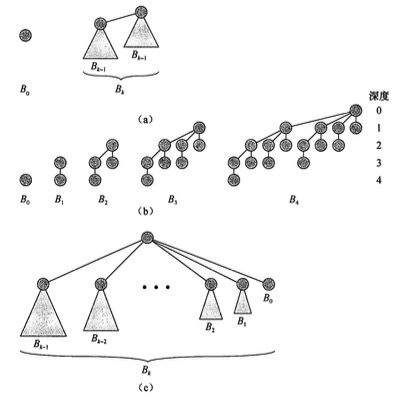
\includegraphics[height=32ex]{1}
    \label{fig:1}
  \end{figure}
  
  \begin{enumerate}[a]
  \item 对于二项树$B_k$, 证明:
    \begin{enumerate}[1]
    \item 一共有$2^k$个结点
    \item 树的高度为$k$
    \item 对于$i=0, 1, \dots, k$, 深度为$i$的节点恰有$\binom{n}{k}$个
    \item 根的度数为$k$, 它比其它任意结点度数都要大。此外, 如果把根的孩子从左到右编号为$k-1, k-2, \dots, 0$, 那么孩子$i$是子树$B_i$的根
    \end{enumerate}

    \begin{addmargin}[3em]{0em}
    使用归纳法:
    \begin{itemize}
    \item 对于$k=0$, 节点个数$n = 1 == 2^k$, 树的高度$h = 1$, 深度为$0$的节点有$\binom{0}{0} = 1$个, 根的度数为$0 == k$。均满足。
    \item 假设对于$k = 0, 1, \dots, m-1$都满足这些性质, 那么对于$k = m$: 由于$B_m$由两个$B_{m-1}$组成。
      \begin{itemize}
      \item 有$n_m = 2 \times n_{m-1} = 2 \times 2^{m-1} = 2^m$
      \item 拼接方法是将某个$B_{m-1}$树接到另一个$B_{m-1}$树的根节点下, 所以新的高度$h_m = 1 + h_{m-1} = m$
      \item $B_{m-1}$树深度为$i$的节点个数为$\binom{m-1}{i}$, 另一棵树$B_{m-1}$接在这棵树的根节点下, 所以这棵树提供的新的深度为$i$的节点个数为$\binom{m-1}{i-1}$,
        有在新的树$B_m$中深度为$i, i=1,2,\dots,m-1$的总节点个数为$\binom{m-1}{i} + \binom{m-1}{i-1} = \binom{m}{i}$;
        深度为0的节点个数仍为$1 = \binom{m-1}{0} == \binom{m}{0}$仍满足性质; 深度为$m$的节点个数为$\binom{m-1}{m-1} = 1 == \binom{m}{m}$也满足该性质;
      \item 根的度数为$1 + \mbox{degree}(B_{m-1}) = m$, 所有其它节点都为曾经合并进的一个更小的树的根节点, 所以它们的度数显然小于$m$。

        已知$B_{m-1}$的$m-1$个孩子分别为$B_{m-2}, B_{m-3}, \dots, B_0$子树的根。当把另外一棵$B_{m-1}$接到这棵树的根节点上构成$B_m$时, 编号为$m-2, m-3, \dots, 0$的子树仍然不变, 所以这些孩子节点仍为$B_{m-2}, B_{m-3}, \dots, B_0$子树的根。对于编号为$m-1$的孩子节点, 就是另外的那棵$B_{m-1}$的子树的根。得证。
      \end{itemize}
    \end{itemize}
    \end{addmargin}

  \item 二项堆$H$是具备如下性质的二项树集合:
    \begin{enumerate}[1]
    \item 每个节点具有一个关键字
    \item $H$中的每个二项树遵循最小堆性质
    \item 对于任意非负整数$k$, $H$中最多有一个二项树的根度数为$k$
    \end{enumerate}
    假定一个二项堆$H$一共有$n$个节点。讨论$H$中包含的二项树与$n$的二进制表示之间的关系。并证明$H$最多由$\lfloor \log(n) \rfloor + 1$棵二项树组成。

    \begin{addmargin}[3em]{0em}
      假设$H$有$n$个节点, 由二项树$B_{l_1}, B_{l_2}, \dots, B_{l_m}$组成, 其中$l_i \geq 0$, 且$l_1 < l_2 < \dots < l_m$有:
      \[
      n = \displaystyle\sum_{i=1}^{i=m} 2^{l_i}
      \]
      所以一定有$n \geq 2^{l_m}$, 其中$B_{l_m}$为其中最大的二项树, 即$l_m \leq \log(n) \implies l_m < \lfloor \log(n) \rfloor + 1$。又由于$H$中对于任意非负整数$k$, $H$中最多只有一个二项树的根度数为$k$, 引入指示变量$b_i$表示$B_i$是否在$H$中, 其中$i = 0, 1, \dots, \lfloor \log(n) \rfloor 1$:
      \[
      n = \displaystyle\sum_{i=1}^{m} 2^{l_i} = \displaystyle\sum_{i=0}{\lfloor \log(n) \rfloor } b_i 2^{i}
      \]
      从上式可以看出若$n$的二进制表达为$b_mb_{m-1}\dotsb_{0}$, 那么对于每个$b_i$为1的位置, $H$就有一颗$B_i$树存在。也可以看出$H$最多由$\lfloor \log(n) \rfloor + 1$棵树组成。
    \end{addmargin}

  \item 假定按如下方式表述二项堆, 用10.4节中的左孩子、右邻兄弟方案来表示二项堆中每一棵二项树。每个节点包含一个关键字, 指向它父节点的指针、指向它最左孩子的指针与它右邻兄弟的指针(这些指针一些情况下是$\mbox{NIL}$), 以及它的度数(如同斐波那契堆, 表示为有多少个孩子)。这些根组成了一个单向链接的根链表, 并以根的度数从小到大排列。可以通过一个指向根链表第一个节点的指针来访问二项堆。

    完整描述如何表示一个二项堆(例如, 对属性进行命名, 描述属性值什么时候为$\mbox{NIL}$, 定义根链表是怎么组织的), 并说明如何用与本章中实现斐波那契一样的方式来实现在二项堆上同样的7个操作。每个操作的最坏时间应该为$O(\log(n))$, 其中$n$为二项堆中的结点数目(或对于$\mbox{UNION}$操作, 为要被合并的两个二项堆中的节点数)。$\mbox{MAKE-HEAP}$操作应为常数时间。

    \begin{addmargin}[3em]{0em}
      二项堆$H$需要维护的属性:
      \begin{itemize}
        \item 指向当前最小二项树的根节点指针$\mbox{min}$
        \item 指向根链表的第一个结点的指针为$\mbox{first}$
        \item 指向根链表最后一个结点的指针为$\mbox{last}$
      \end{itemize}

      每个节点$u$的属性如下:
      \begin{itemize}
      \item $\mbox{key}$: 关键字
      \item $\mbox{degree}$: 度数/该节点孩子节点的个数
      \item $p$: 指向父亲节点的指针
      \item $\mbox{child}$: 指向最左孩子节点的指针
      \item $\mbox{right}$: 指向右邻兄弟节点的指针
      \item $\mbox{last}$: 指向根链表中上一个节点的指针
      \item $\mbox{next}$: 指向根链表中的下一个节点的指针
      \end{itemize}

    七个操作如下:
    \begin{algorithm}[H]
      \caption{MAKE-HEAP()}
      \begin{algorithmic}
        \State{allocate an object H}
        \State $H.\mbox{first} = \mbox{NIL}$
        \State $H.\mbox{last} = \mbox{NIL}$
        \State $H.\mbox{min} = \mbox{NIL}$
        \State\Return $H$
      \end{algorithmic}
    \end{algorithm}

    \begin{algorithm}[H]
      \caption{HEAP-INSERT($H$, $x$)}
      \begin{algorithmic}
        \State $x.\mbox{degree}=0, x.p = \mbox{NIL}$
        \State $x.\mbox{child}=\mbox{NIL}, x.\mbox{right} = \mbox{NIL}$\Comment{新的节点没有兄弟或者子孙节点}
        \State $x.\mbox{next}=H.\mbox{first}$
        \State $H.\mbox{first} = x$
        \State $\mbox{CONSOLIDATE}(H)$\Comment{维持二项堆的每个度数的树最多只有一个的性质}
      \end{algorithmic}
    \end{algorithm}

    \begin{algorithm}[H]
      \caption{CONSOLIDATE($H$)}
      \begin{algorithmic}
        \State $d = \lfloor \log(n) \rfloor$
        \State{let $A[0,\dots,d]$ be a new array}
        \For{$i=0 .. d$}
        \State $A[i] = \mbox{NIL}$
        \EndFor
        \For{each node $w$ in the root list of $H$}
        \State $x = w, d = x.\mbox{degree}$
        \While{$A[d] != \mbox{NIL}$}
        \State $y = A[d]$
        \If{$x.\mbox{key} > y.\mbox{key}$}
        \State{exchange $x$ and $y$}
        \EndIf
        \State $\mbox{HEAP-LINK}(H, y, x)$
        \State $A[d] = \mbox{NIL}$
        \State $d = d+1$
        \EndWhile
        \State $A[d] = x$
        \EndFor
        \State $H.\mbox{first} = \mbox{NIL}$
        \State $\mbox{last} = \mbox{NIL}$
        \For{$i=0 .. d$}
        \If{$A[i]!=\mbox{NIL}$}
        \If{$\mbox{last} == \mbox{NIL}$}
        \State $A[i].\mbox{last} = \mbox{last}$
        \State $H.\mbox{first} = \mbox{last} = A[i]$
        \State $H.\mbox{min} = A[i]$
        \Else
        \State $A[i].\mbox{last} = \mbox{last}$
        \State $\mbox{last}.\mbox{right}=A[i]$
        \State $\mbox{last} = A[i]$
        \If{$A[i].\mbox{key} < H.\mbox{min}.\mbox{root}.\mbox{key}$}\Comment{根据需要更新$H.\mbox{min}$指针}
        \State $H.\mbox{min} = A[i]$
        \EndIf
        \EndIf
        \EndIf
        \EndFor
      \end{algorithmic}
    \end{algorithm}

    \begin{algorithm}[H]
      \caption{HEAP-LINK($H$, $y$, $x$)}
      \begin{algorithmic}
        \If{$y.\mbox{last} == \mbox{NIL}$}\Comment{remove $y$ from the root list of $H$}
        \State $H.\mbox{first} = y.\mbox{next}$
        \Else
        \State $y.\mbox{last}.\mbox{next} = y.\mbox{next}$
        \EndIf
        \Comment{make $y$ a child of $x$, incrementing $x.\mbox{degree}$}
        \State $y.\mbox{next} = \mbox{NIL}, y.\mbox{last} = \mbox{NIL}$
        \State $y.\mbox{right} = x.\mbox{child}$
        \State $x.\mbox{child} = y$
        \State $y.p = x$
        \State $x.\mbox{degree} += 1$
      \end{algorithmic}
    \end{algorithm}

    \begin{algorithm}[H]
      \caption{HEAP-UNION($H_1$, $H_2$)}
      \begin{algorithmic}
        \State $H_1.\mbox{last}.\mbox{next} = H_2.\mbox{first}$
        \State $H_2.\mbox{first}.\mbox{last} = H_1.\mbox{last}$
        \If{$H_1.\mbox{min} == \mbox{NIL} \lor (H_2.\mbox{min} != NIL land H_2.\mbox{min}.\mbox{key} < H_1.\mbox{min}.\mbox{key})$}
        \State $H_1.\mbox{min} = H_2.\mbox{min}$
        \State $\mbox{CONSOLIDATE}(H_1)$ \Comment{维护二项堆性质}
        \EndIf
        \State\Return $H_1$
      \end{algorithmic}
    \end{algorithm}

    \begin{algorithm}[H]
      \caption{HEAP-EXTRACT-MIN($H_1$, $H_2$)}
      \begin{algorithmic}
        \State $z=H.\mbox{min}$
        \State{remove $z$ from the root list of $H$}\Comment{具体的链表操作与上面$\mbox{HEAP-LINK}$中类似, 不再详细写出}
        \If{$z != \mbox{NIL}$}
        \For{each child $x$ of $z$}
        \State $x.p = \mbox{NIL}$
        \State{add $x$ to the root list of $H$}
        \EndFor
        \EndIf
        \State $\mbox{CONSOLIDATE}(H)$
        \State\Return $z$
      \end{algorithmic}
    \end{algorithm}

    \begin{algorithm}[H]
      \caption{HEAP-DECREASE-KEY($H$, $x$, $k$)}
      \begin{algorithmic}
        \If{$k > x.\mbox{key}$}
        \State{error}
        \EndIf
        \State $x.\mbox{key} = k$
        \While{$x.p != \mbox{NIL}$}
        \State{remove $x$ from this tree and add $x$ into the root list of $H$}
        \EndWhile
        \State $\mbox{Consolidate}(H)$
      \end{algorithmic}
    \end{algorithm}

    \begin{algorithm}[H]
      \caption{DELETE($H$, $x$)}
      \begin{algorithmic}
        \State $\mbox{HEAP-DECREASE-KEY}(H, x, -\inf)$
        \State $\mbox{HEAP-EXTRACT-MIN}(H)$
      \end{algorithmic}
    \end{algorithm}
    \end{addmargin}

  \item 假定仅仅要是现在一个斐波那契堆上的可合并堆操作(不实现$\mbox{DECREASE-KEY}$和$\mbox{DELETE}$操作)。斐波那契堆中的树与二项堆中的树有何相似之处? 有什么区别? 证明在一个$n$节点的斐波那契堆中最大度数最多为$\lfloor \log(n) \rfloor$.
  \begin{addmargin}[3em]{0em}
    相似之处:
    \begin{itemize}
    \item $\mbox{EXTRACT-MIN}$过程后两个数据结构均满足性质: 对于任何度数, 最多只有一个树为该度数
    \item 两个堆都是由多个树组成的, 且这些树都满足最小堆性质
    \end{itemize}
    区别在于斐波那契堆并不是在任何时候都满足对于任何度数, 最只有多一个树为该度数; 但是在我的二项堆实现中, 各种操作都调用了$\mbox{Consolidate}$维持该性质。且斐波那契堆中的树的结构和二项堆中树的结构并不一样。

    课上已经证明对于斐波那契堆中的任意一棵树$x$, $k = x.\mbox{degree}$有:
    \[
    \mbox{size}(x) \geq F_{k+2} \geq \phi^k
    \]
    其中$\phi = \frac{1 + \sqrt{5}}{2}$, 又有$\mbox{size}(x) \leq n$, 可得: $k \leq \log_\phi (n)$.
  \end{addmargin}

\item McGee教授提出了一个基于斐波那契堆的新数据结构, 一个McGee堆具有与斐波那契堆相同的结构, 并且只支持可合并堆操作。除了插入和合并在最后一步中合并根链表外, 其它操作的实现方式均与斐波那契堆中的实现方式相同。McGee堆上各操作的最坏情况运行时间为多少?

  为啥我觉得跟斐波那契堆一样啊...
  \end{enumerate}

\section{Problem 2}
\textbf{22.1-7. 有向无环图$G=(V, E)$的关联矩阵是一个满足下述条件的$|V| \times |E|$的矩阵$B=(b_{ij})$:}
\[
b_{ij} =
\begin{cases}
  -1 & \quad \text{如果边$j$从节点$i$发出}\\
  1 & \quad \text{如果边$j$进入节点$i$}\\
  0 & \quad \text{其它}
\end{cases}
\]
\textbf{请说明矩阵乘积$BB^T$里的每个元素代表什么意思。这里$B^T$是矩阵$B$的转置。}

$C = BB^T \implies c_{ij} = \sum_k {b_{ik} b_{jk}}$

即每个元素$c_{ij}$代表: 初始化为0, 考察$i$, $j$以外的每个节点$k$:
\begin{itemize}
\item 若$k$节点和$i$, $j$中有一个没有连接, $c_{ij}$不变
\item 若$k$节点和$i$, $j$连接方向一致, $c_{ij}$增加1
\item 若$k$节点和$i$, $j$连接方向相反, $c_{ij}$减少1
\end{itemize}

\section{Problem 3}
\textbf{22.2-7. 职业摔跤手分为两种类型: ``娃娃脸''(``好人'')型和``高跟鞋''(``坏人'')型。在任意一对职业摔跤手之间都可能存在竞争关系。假定有$n$个职业摔跤手, 并且有一个给出竞争关系的$r$对摔跤手的链表。给出一个$O(n+r)$的算法判断是否可以将某些摔跤手分为``娃娃脸'', 而剩下的分为``高跟鞋''型, 使得所有竞争关系均只存在于娃娃脸型和高跟鞋型选手之间。如果可以进行这种划分, 则算法还应当生成一种这样的划分。}

这很明显是一个二分图问题, 竞争关系表为边集$E$, 职业摔跤手集合为顶点集$V$, 在图$G=(V, E)$中找到一个划分(``cut''), 使得所有边全部切割这个cut。我们可以使用深度优先遍历的算法实现这个过程, 由于这是一个无向图, 深度优先遍历过程中只会生成tree edge或者back edge。 我们只需要在遍历的时候沿着tree edge交替分配不同型号, 并在发现back edge的时候查看是否这条边两边的顶点仍然满足型号不同即可。算法如下:
  \begin{algorithm}[H]
    \caption{BI-PARTIE($G$)}
    \label{algo:1}
    \begin{algorithmic}
      \For{each vertex} $u \in G.V$
      \State $u.\mbox{color} = \mbox{WHITE}$
      \EndFor
      \For{each vertex} $u \in G.V$
      \If{$u.\mbox{color} == \mbox{WHITE}$}
      \State $\mbox{yes} = \mbox{VISIT}(u, 0)$
      \If{$!\mbox{yes}$}
      \State\Return $\mbox{false}$
      \EndIf
      \EndIf
      \EndFor
      \State\Return $\mbox{true}$
    \end{algorithmic}

  \end{algorithm}
    \begin{algorithm}[H]
    \caption{VISIT($u$, $\mbox{label}$)}
    \begin{algorithmic}
      \State $u.\mbox{label} = \mbox{label}$
      \State $\mbox{label} = 1 - \mbox{label}$
      \State $u.\mbox{color} = \mbox{GRAY}$
      \For{each vertex} $u \in G.\mbox{Adj}[u]$
      \If{$v.\mbox{color} == \mbox{WHITE}$}
      \State $\mbox{yes} = \mbox{VISIT}(v, \mbox{label})$
      \If{$!\mbox{yes}$}\Comment{某个子节点无法成功划分}
      \State\Return $\mbox{false}$
      \EndIf
      \Else\Comment{肯定为$\mbox{GRAY}$}
      \If{$v.\mbox{label} == u.\mbox{label}$}
      \Return $\mbox{false}$\Comment{这个节点与其祖先节点冲突, 无法成功划分}
      \EndIf
      \EndIf
      \EndFor
      \State $u.\mbox{color} = \mbox{BLACK}$
      \State\Return $\mbox{true}$
    \end{algorithmic}
  \end{algorithm}

\end{document}
